\documentclass{beamer}
%\documentclass[handout]{beamer}
%\usepackage{pgfpages}
%\pgfpagesuselayout{4 on 1}[a4paper,border shrink=5mm,landscape]
\usepackage[italian]{babel}
\usepackage[utf8]{inputenc}
\usepackage[T1]{fontenc}
\usepackage{lmodern}
\usepackage{verbatim}
\usepackage{amsmath}
\usepackage{amsfonts}
\usepackage{amssymb}
\usepackage{graphicx}
\usepackage{listings}
\usepackage{hyperref}
\usepackage{multirow}

\definecolor{mygray}{rgb}{0.5,0.5,0.5}
\definecolor{RaspberryPi}{HTML}{BB1142}

\usetheme{Pittsburgh}
\setbeamercovered{dynamic}
\setbeamertemplate{frametitle}[default][left]

\setbeamercolor{structure}{fg=RaspberryPi}
%\setbeamercolor{frametitle}{fg=OpenStack}
%\setbeamercolor{title in head/foot}{fg=OpenStack}
%\setbeamercolor{author in head/foot}{fg=blue!55!black}
%\setbeamercolor{date}{fg=blue!40!black}
%\setbeamercolor{institute in head/foot}{fg=blue!55!black}
%\setbeamercolor{section in head/foot}{fg=blue!55!black}

\setbeamertemplate{sidebar canvas right}{\vspace*{3pt}\hspace*{-93pt}{
\includegraphics[angle=0,origin=c,height=40pt]{imgs/logo02.png}}}
\beamertemplatenavigationsymbolsempty


\begin{document}


\begin{frame}[plain]
\begin{center}

\includegraphics[width=0.08\textwidth]{imgs/logo-uniroma2-red.png}
\\    
\textbf{\color{RaspberryPi} Università  degli studi di \\Roma Tor Vergata}
\\[0.2cm]
\tiny Facoltà di Ingegneria
\\[0.2cm]
\small Roma2LUG
\\
\tiny Linux User Group
\\[0.2cm]


\vfill
{
\Large \textbf{Roma2LUG Incontra}
\\[0.2cm]
\color{RaspberryPi}\Large \textbf{Music On Linux}
\\[1.0cm]
}
\vfill

\small{
\textbf{Speaker}
\hfill
\textbf{Speaker}
\\
\textit{Giulia Cassarà}
\hfill
\textit{Emanuele Savo}}


\end{center}

\end{frame}


%\begin{frame}
%\frametitle{\textbf{Indice della presentazione}}
%\framesubtitle{Argomenti trattati}
%\tableofcontents
%\end{frame}

\lstdefinestyle{customc}{
  belowcaptionskip=1\baselineskip,
  breaklines=true,
  %language=BASH,
  showstringspaces=false,
  frame=none,
  basicstyle=\small\ttfamily,
  keywordstyle=\bfseries\color{blue},
  commentstyle=\itshape\color{red},
  stringstyle=\color{orange},
  rulecolor=\color{black}
}

\lstset{escapechar=@,style=customc}


%Inizio presentazione

\begin{frame}
\frametitle{\textbf{Raspberry Pi}}
\framesubtitle{\textbf{Introduction to the Raspberry Pi 3 Model B Board}}
\begin{figure}
\centering
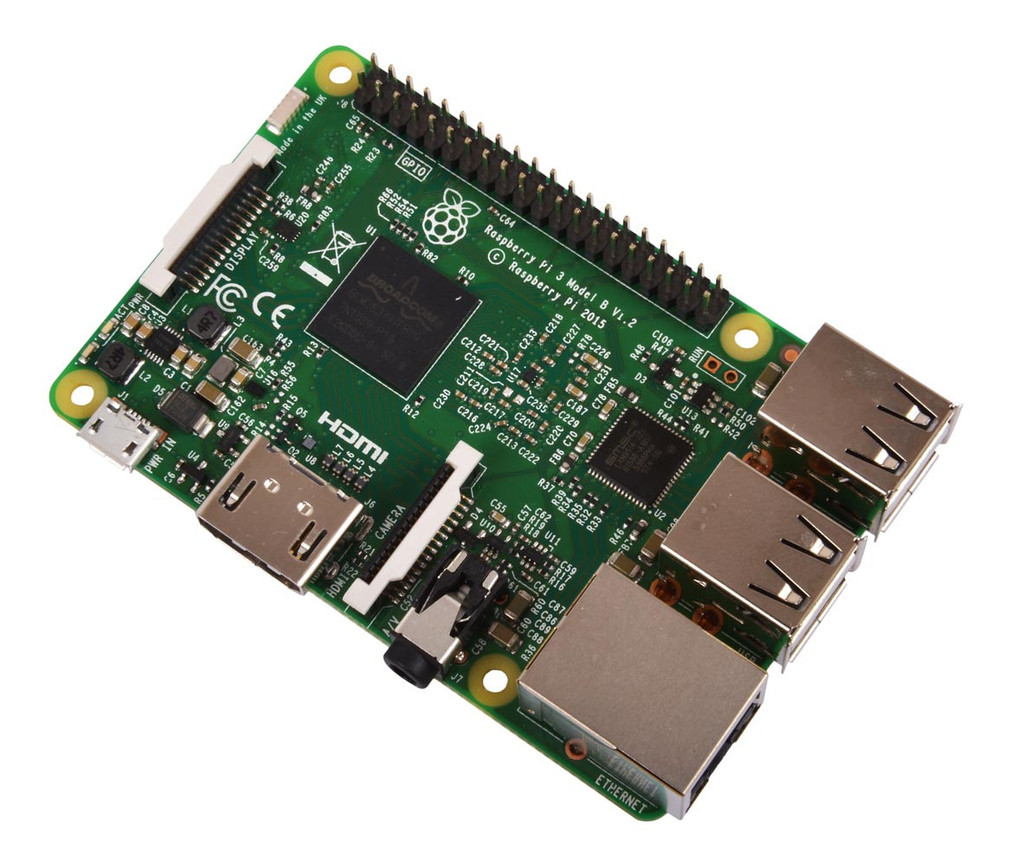
\includegraphics[scale=0.15]{imgs/rasp3b.jpg}
\begin{block}{General features}
\begin{itemize}
\item[$\bullet$] Born as a MiniPC
\item[$\bullet$] Can reproduce HD movies
\item[$\bullet$] The main difference with a PC are the GPIO ports
\end{itemize}
\end{block}
\end{figure}
\end{frame}

%%%%%%%%%%%%%%%%%%%%%

\begin{frame}
\frametitle{\textbf{Raspberry Pi}}
\framesubtitle{\textbf{Specs of the Raspberry Pi 3 Model B Board}}
\begin{figure}
\centering
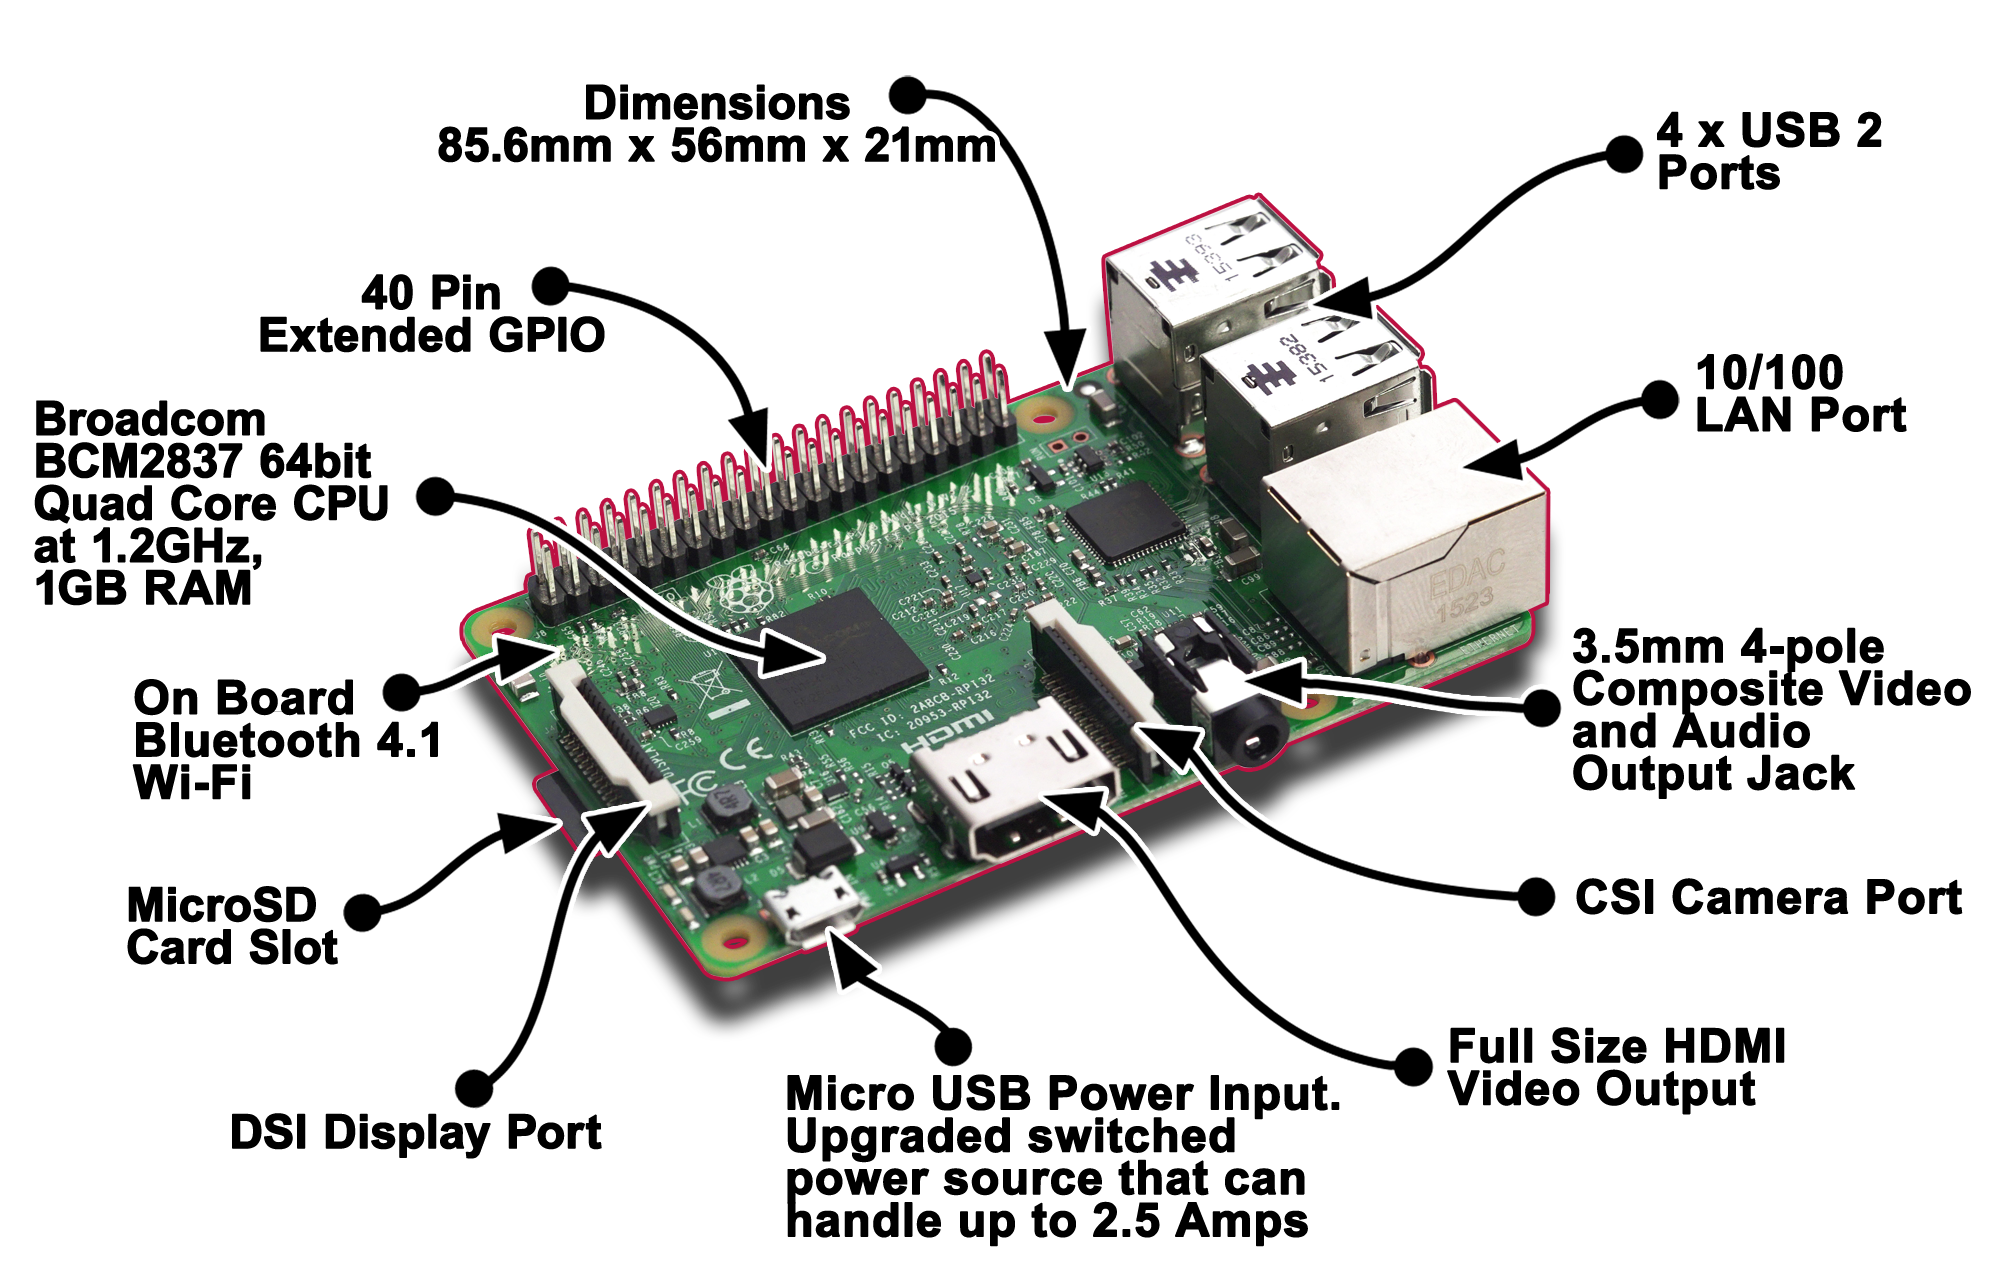
\includegraphics[scale=0.70]{imgs/rasp3btec.png}
\end{figure}
\end{frame}

%%%%%%%%%%%%%%%%%%%%%%

\begin{frame}
\frametitle{\textbf{Raspberry Pi}}
\framesubtitle{\textbf{GPIO ports mapping of the Raspberry Pi 3 Model B Board}}
\begin{figure}
\centering
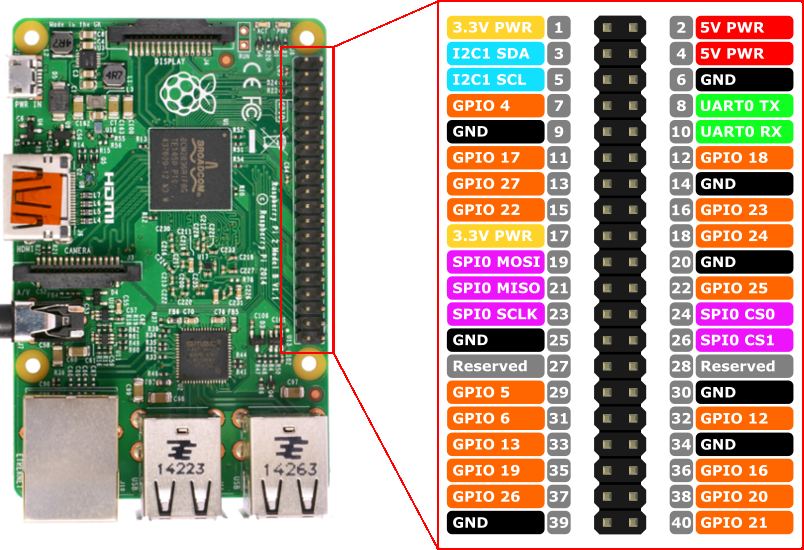
\includegraphics[scale=1]{imgs/gpio.png}
\end{figure}
\end{frame}

%%%%%%%%%%%%%%%%%%%%%%%%%%%%%%

\begin{frame}[fragile]
\frametitle{\textbf{Raspbian OS installation}}
\framesubtitle{\textbf{Download and unzip OS}}

\begin{center}

\includegraphics[width=0.60\textwidth]{imgs/raspbian_logo.jpg}
\end{center}
\begin{itemize}
\item[$\bullet$] Download Raspbian OS lite version for the Raspberry Pi
\begin{lstlisting}
  $ wget https://downloads.raspberrypi.org/raspbian_lite_latest
\end{lstlisting}
\item[$\bullet$] Unzip Raspbian OS for the Raspberry Pi
\begin{lstlisting}
  $ unzip xxxx-xx-xx-raspbian-jessie-lite.zip
\end{lstlisting}
\end{itemize}

\end{frame}

%%%%%%%%%%%%%%%%%%%%%%%%%%%%%%%

\begin{frame}[fragile]
\frametitle{\textbf{After Download}}
\framesubtitle{\textbf{Prepare SD card}}
\begin{itemize}
\item[$\bullet$] Insert SD card into the PC
\item[$\bullet$] Search for device name of the SD card with this command:
\begin{lstlisting}
  $ sudo fdisk -l
\end{lstlisting}
\item[$\bullet$] Search for info about your SD card. \textit{Warning, be careful!}
\begin{lstlisting}[basicstyle=\tiny\ttfamily]
  Disk /dev/mmcblk0: 14,5 GiB, 15523119104 bytes, 30318592 sectors      
  Units: sectors of 1 * 512 = 512 bytes                                 
  Sector size (logical/physical): 512 bytes / 512 bytes                 
  I/O size (minimum/optimal): 512 bytes / 512 bytesa                    
  Disklabel type: dos                                                   
  Disk identifier: 0x6f92008e                                           
\end{lstlisting}
\item[$\bullet$] Replace mmcblk0 with device name of your SD
\begin{lstlisting}
  $ sudo dd \
    if=/xxxx-xx-xx-raspbian-jessie-lite.img \
    of=/dev/mmcblk0
\end{lstlisting}
\end{itemize}

\end{frame}

%%%%%%%%%%%%%%%%%%%%%%%%%%%%%%

\begin{frame}[fragile]
	\frametitle{\textbf{Boot}}
	\framesubtitle{\textbf{Boot the system and update packages}}

		\begin{itemize}
			\item[$\bullet$] Connect ethernet cable to the Raspberry Pi
			\item[$\bullet$] Connect HDMI cable to the Raspberry Pi
			\item[$\bullet$] Connect micro USB power cable to the Raspberry Pi
			\item[$\bullet$] Waiting for complete boot...
			\item[$\bullet$] Login
			\begin{itemize}
				\item[$\bullet$] user: pi
				\item[$\bullet$] password: raspberry
			\end{itemize}
			\item[$\bullet$] Execute these commands:
			\begin{lstlisting}
  $ sudo apt-get update
  $ sudo apt-get dist-upgrade -y
  $ sudo apt-get install rpi-upate -y
			\end{lstlisting}
		\end{itemize}
\end{frame}

%%%%%%%%%%%%%%%%%%%%%%%%%%%%%%%

\begin{frame}[fragile]
	\frametitle{\textbf{Configuration}}
	\framesubtitle{\textbf{Expand filesystem and configure your raspberry}}
		\begin{itemize}
			\item[$\bullet$] Config Raspbian OS with this tool
			\begin{lstlisting}
   $ sudo raspi-config
			\end{lstlisting}
			\begin{itemize}
				\item[$\bullet$] Expand Filesystem
				\item[$\bullet$] Internationalisation Options
				\begin{itemize}
					\item[$\bullet$] Change Locale
					\item[$\bullet$] Change Timezone
					\item[$\bullet$] Change Keyboard Layout
					\item[$\bullet$] Change wifi Country
				\end{itemize}
			\end{itemize}
			\begin{lstlisting}
   $ sudo reboot
			\end{lstlisting}
			\item[$\bullet$] Update Raspberry Pi firmware
			\begin{lstlisting}
   $ sudo rpi-update
   $ sudo reboot
			\end{lstlisting}
		\end{itemize}
\end{frame}

%%%%%%%%%%%%%%%%%%%%%%%%%%%%%%

\begin{frame}[fragile]
	\frametitle{\textbf{WiringPi and GIT}}
	\framesubtitle{\textbf{Install necessary software}}
		\begin{itemize}
			\item[$\bullet$] Install library for gpio and other tools
			\begin{lstlisting}
  $ sudo apt-get install -y wiringpi git vim
			\end{lstlisting}
			\item[$\bullet$] Download the scripts
			\begin{lstlisting}
  $ git clone https://github.com/Roma2Lug-Projects/MusicOnLinux.git
			\end{lstlisting}
			\item[$\bullet$] Open the script
			\begin{lstlisting}
  $ cd MusicOnLinux/Scripts
  $ vim keyboard.sh
  $ vim smario.sh
			\end{lstlisting}
		\end{itemize}
\end{frame}

%%%%%%%%%%%%%%%%%%%%%%%%%%%%%%%

\begin{frame}[fragile]
	\frametitle{\textbf{Final steps}}
	\framesubtitle{\textbf{Script's permission and execution}}

		\begin{itemize}
			\item[$\bullet$] Give execute permission
			\begin{lstlisting}
  $ chmod +x keyboard.sh
  $ chmod +x smario.sh
			\end{lstlisting}
			\item[$\bullet$] Execute the scripts!
			\begin{lstlisting}
  $ ./keyboard.sh
  $ ./smario.sh
			\end{lstlisting}
		\end{itemize}
\end{frame}


%%%%%%%%%%%%%%%%%%%%%%%%%%%%%%%

\begin{frame}[fragile]
	\frametitle{\textbf{Tone function}}
			\begin{lstlisting}[language=bash]
#! /bin/bash
tone () {
  local note="$1"
  local duration="$2"
  if test "$note" -eq 0; then
    gpio -g mode 18 in
  else
    local period=$(python -c "print '{0:.0f}'.format(600000.0/440.0/2**(($note-69)/12.0))")
    gpio -g mode 18 pwm
    gpio pwmr "$(( period ))"
    gpio -g pwm 18 "$(( period/2 ))"
    gpio pwm-ms
    sleep $duration
    tone 0
  fi
}

			\end{lstlisting}
\end{frame}


%%%%%%%%%%%%%%%%%%%%%%%%%%%%%%%

\begin{frame}[fragile]
	\frametitle{\textbf{Tone function in details (1)}}
  \begin{lstlisting}[language=bash]
  tone () {
    local note="$1"
    local duration="$2"
    if test "$note" -eq 0; then
      gpio -g mode 18 in
    ...
  \end{lstlisting}
  \begin{itemize}
  	\item[$\bullet$] First parameter: note.
  	\item[$\bullet$] Second parameter: duration of the note.
  	\item[$\bullet$] Test if the note is 0 then put the GPIO in input mode, so the speaker doesn’t make any sound. 
  \end{itemize}
\end{frame}

%%%%%%%%%%%%%%%%%%%%%%%%%%%%%%%

\begin{frame}[fragile]
	\frametitle{\textbf{Tone function in details (2)}}
  \begin{lstlisting}[language=bash]
    ...
    else
      local period=$(python -c "print '{0:.0f}'.format(600000.0/440.0/2**(($note-69)/12.0))")
      ...
  \end{lstlisting}
  \begin{itemize}
  	\item[$\bullet$] We use the formula below to obtain the frequency of the speaker
  	
  	\begin{center}
  			$K\cdot\frac{440}{2^{\frac{X-69}{12}}}$
  	\end{center}
  		
  	
  	\item[$\bullet$] $K =\frac{19.2MhZ}{32} = 600khZ$ is the base frequency of the speaker where 19.2MhZ is the speed of the raspberry internal clock.
  	\item[$\bullet$] The twelfth root of two or $\sqrt[12]{2}$ is an algebraic irrational number. It is most important in music theory, where it represents the frequency ratio of a semitone in twelve-tone equal temperament.
  	\item[$\bullet$] X is the range of the note, encoded in ASCII.
  \end{itemize}
\end{frame}

%%%%%%%%%%%%%%%%%%%%%%%%%%%%%%%


\begin{frame}[fragile]
	\frametitle{\textbf{Tone function in details (3)}}
  \begin{lstlisting}[language=bash]
      ...
      gpio -g mode 18 pwm
      gpio pwmr "$(( period ))"
      gpio -g pwm 18 "$(( period/2 ))"
      gpio pwm-ms
      sleep $duration
      tone 0
    fi
  }
  \end{lstlisting}
  \begin{itemize}
  \item[$\bullet$] This is the core of the function. These lines of code give power to the connected speaker with a modulation technique called Pulse Width Modulation (PWM).
  \item[$\bullet$] The speaker beeps the "note" for a time "duration".
  \item[$\bullet$] Finally the last command mute the sound by recalling the tone function with 0. Without this line the speaker will sound indefinitily(!!!).
  \end{itemize}
\end{frame}

%%%%%%%%%%%%%%%%%%%%%%%%%%%%%%%


\begin{frame}[plain]
\begin{center}

\includegraphics[width=0.12\textwidth]{imgs/logo-uniroma2-red.png}
\vfill
\huge{\textit{\textbf{[DEMO]}}}
\vfill

\includegraphics[width=0.40\textwidth]{imgs/logo02.png}
\end{center}
\end{frame}

%%%%%%%%%%%%%%%%%%%%%%%%%%%%%%%


\begin{frame}[plain]
\begin{center}

\includegraphics[width=0.12\textwidth]{imgs/logo-uniroma2-red.png}
\vfill
\huge{\textit{\textbf{Grazie per l'attenzione!}}}
\vfill

\includegraphics[width=0.40\textwidth]{imgs/logo02.png}
\end{center}
\end{frame}

\end{document}